% =====================================================================
%  IEEE-STYLE CONFERENCE REPORT TEMPLATE  (self-contained)
%  MLE-AI-201 Machine Learning -- Final Project
%
%  This template MIMICS the IEEE two-column conference look using only
%  standard LaTeX packages. It does NOT depend on IEEEtran.cls, so it
%  compiles anywhere (tectonic, pdflatex, Overleaf) with nothing extra.
%
%  Build:   tectonic report.tex      (recommended)
%     or:   pdflatex report.tex ; pdflatex report.tex
% =====================================================================
\documentclass[10pt,twocolumn,a4paper]{article}

% ---- Geometry: IEEE-like margins / two narrow columns ----------------
\usepackage[a4paper,top=0.75in,bottom=1.0in,left=0.68in,right=0.68in,columnsep=0.25in]{geometry}

% ---- Times-like font (standard, ships with every TeX distro) ---------
\usepackage{mathptmx}          % Times text + math
\usepackage[T1]{fontenc}
\usepackage[utf8]{inputenc}    % allows accented / Azerbaijani chars

% ---- Common, dependency-free packages --------------------------------
\usepackage{graphicx}
\usepackage{amsmath,amssymb}
\usepackage{booktabs}
\usepackage{array}
\usepackage{titlesec}
\usepackage{caption}
\usepackage{cite}
\usepackage[hidelinks]{hyperref}
\usepackage{url}

% ---- IEEE-style section headings -------------------------------------
\renewcommand{\thesection}{\Roman{section}}
\renewcommand{\thesubsection}{\Alph{subsection}}
\titleformat{\section}[block]{\centering\normalsize\scshape}{\thesection.}{0.5em}{}
\titleformat{\subsection}[block]{\normalsize\itshape}{\thesubsection.}{0.5em}{}
\titlespacing*{\section}{0pt}{1.4ex plus 1ex minus .2ex}{1ex}
\titlespacing*{\subsection}{0pt}{1.0ex plus 1ex minus .2ex}{0.6ex}

% ---- Abstract / Index-Terms in the IEEE boldface-dash style ----------
\newcommand{\abstractkw}[1]{\noindent\textbf{\textit{#1}}}

\captionsetup{font=small,labelsep=period}
\setlength{\parindent}{1em}

% =====================================================================
\begin{document}

% ------------------------- TITLE BLOCK --------------------------------
\twocolumn[
  \begin{@twocolumnfalse}
  \begin{center}
    {\LARGE\bfseries Your Project Title Here:\\A Clear, Specific Subtitle\par}
    \vspace{1.2em}
    % Authors: Surname, Given name --- alphabetical by surname.
    {\large
      Aliyeva, Aysel\quad Mammadov, Murad\quad Rustamli, Rustam\par}
    \vspace{0.5em}
    {\itshape MLE-AI-201 Machine Learning, AI Academy --- Cohort II\par}
    \vspace{1.4em}
  \end{center}
  \begin{quote}
    \small
    \abstractkw{Abstract---}% IEEE uses an em-dash after "Abstract"
    One paragraph, roughly 150--250 words. State the problem (price
    prediction and the derived price-tier task on the bina.az dataset),
    what you built from scratch (a decision tree and an SVM), the key
    result (headline metrics vs.\ scikit-learn), and the main takeaway.
    Write it last. \textbf{End the abstract with your repository link},
    per IEEE convention:
    \href{https://github.com/your-team/your-repo}{\texttt{github.com/your-team/your-repo}}
    (tag \texttt{v1.0-final}).

    \vspace{0.6em}
    \abstractkw{Index Terms---}decision tree, support-vector machine,
    Pegasos, regression, classification, real-estate price prediction.
  \end{quote}
  \vspace{1.0em}
  \end{@twocolumnfalse}
]

% =====================================================================
\section{Introduction}
Motivate the problem and state your contributions as a short bulleted or
inline list. What is the task, why does it matter, and what did your
team do? Keep background brief; cite sources like this~\cite{pegasos}.

\section{Related Work / Background}
Briefly place your work in context: decision trees (impurity, information
gain), the soft-margin SVM and the hinge-loss primal, and the Pegasos
sub-gradient solver you used~\cite{pegasos}. One or two short paragraphs.

\section{Data and Preprocessing}
Describe the bina.az dataset: size, key columns, and the cleaning you
did (currency, types, missing values, duplicates, outliers). State the
two tasks (price regression; price-tier classification), how you derived
the tier label, and your train/validation/test split. \textbf{Name the
leakage columns you removed and why.}

\begin{table}[t]
  \centering
  \caption{Dataset summary after cleaning.}
  \label{tab:data}
  \begin{tabular}{@{}lr@{}}
    \toprule
    Property & Value \\
    \midrule
    Rows (after cleaning)       & 64,454 \\
    Features used               & 5 \\
    Train / Val / Test split    & 45,118 / 9,667 / 9,669 \\
    Premium share (train)       & 49.5\% \\
    \bottomrule
  \end{tabular}
\end{table}

\section{Method}
\subsection{Decision tree (from scratch)}
Describe your impurity criteria (Gini / entropy / MSE reduction), the
split search, recursion, leaf rule, and hyperparameters.

\subsection{Support-vector machine (from scratch)}
We map the standard and premium labels to $-1$ and $+1$, respectively,
and minimize the regularized hinge-loss objective:
\begin{equation}
  J(\mathbf{w},b)=\tfrac{\lambda}{2}\lVert\mathbf{w}\rVert^{2}
  +\tfrac{1}{n}\sum_{i=1}^{n}\max\!\big(0,\,1-y_i(\mathbf{w}^{\top}\mathbf{x}_i+b)\big).
\end{equation}
For the linear model, the margin width is $2/\lVert\mathbf{w}\rVert_2$.
We identify training points on or inside the margin as support vectors:
\begin{equation}
  y_i(\mathbf{w}^{\top}\mathbf{x}_i+b)\leq 1.
\end{equation}
At update $t$, Pegasos samples training example $i_t$ and uses
$\eta_t=1/(\lambda t)$. Its stochastic updates are
\begin{align}
  \mathbf{w}_t &= (1-\eta_t\lambda)\mathbf{w}_{t-1}
    +\eta_t y_{i_t}\mathbf{x}_{i_t}\,
      \mathbb{1}\!\left[y_{i_t}(\mathbf{w}_{t-1}^{\top}\mathbf{x}_{i_t}
      +b_{t-1})<1\right],\\
  b_t &= b_{t-1}+\eta_t y_{i_t}\,
      \mathbb{1}\!\left[y_{i_t}(\mathbf{w}_{t-1}^{\top}\mathbf{x}_{i_t}
      +b_{t-1})<1\right].
\end{align}
The bias is unregularized: it is updated on margin violations but is not
multiplied by the weight-decay factor. For the nonlinear model, random
Fourier features approximate an RBF kernel:
\begin{equation}
  \begin{aligned}
    \mathbf{z}(\mathbf{x}) &= [z_j(\mathbf{x})]_{j=1}^{D},\\
    z_j(\mathbf{x}) &= \sqrt{\tfrac{2}{D}}\cos(\phi_j(\mathbf{x})),\\
    \phi_j(\mathbf{x}) &= \boldsymbol{\omega}_j^{\top}\mathbf{x}+c_j,\\
    \boldsymbol{\omega}_j &\sim \mathcal{N}(0,2\gamma\mathbf{I}),\\
    c_j &\sim \mathcal{U}(0,2\pi), \quad j=1,\ldots,D.
  \end{aligned}
\end{equation}
Pegasos is applied to $\mathbf{z}(\mathbf{x})$; its transformed-space
coefficients are not interpreted as original-feature importance.

\section{Experimental Setup}
All experiments used seed 42. After deduplication, 70\% of the rows were
reserved for training. The premium threshold was set to the training
price median; the remaining rows were split into validation and test
halves stratified by that label. Missing numeric features were filled
with training medians. The team's SVM used training means and standard
deviations; scikit-learn's hinge-loss baseline scaled features inside
a pipeline. Every cross-validation fold refitted its own preprocessing
on that fold's training rows.

Tree depth, minimum leaf size, Gini versus entropy, SVM regularisation,
and RFF bandwidth were chosen from validation results only. The regression
selection metric was log-RMSE; classification used premium-class F1.
The test rows were evaluated once with the selected settings. We report
price-scale RMSE, MAE, and $R^2$, plus precision, recall, F1, ROC-AUC,
and confusion matrices for price tiers. NumPy implementations computed
the metrics. We compared the trees with matched scikit-learn trees and
the linear Pegasos SVM with a scaled SGD hinge-loss classifier. Wall-clock
fit and prediction times were measured separately and recorded by the
reproduction script; they depend on the machine.

\subsection{SVM protocol}
We used the deterministic split with seed 42. Missing feature values were
imputed using training-set medians, the premium threshold was the median
training price, and a $\texttt{StandardScaler}$ was fitted on training
features only and then applied to validation features. The five numeric
inputs were area, floor number, total floors, latitude, and longitude.
Both models used the same transformed training and validation partitions.
Linear Pegasos used $\lambda=0.01$, $3n_{\mathrm{train}}$ updates, and
seed 42. The RFF model used $\gamma=1$, $D=500$, $\lambda=10^{-4}$,
20,000 updates, and seed 42. Reported model metrics and error analyses
below are validation results. The convergence trace uses the training
objective, recorded every 1,000 updates during one 20,000-update run with
$\lambda=0.01$.

\section{Results}
The reproducible run retained 64,454 unique listings. The seeded split
contained 45,118 training, 9,667 validation, and 9,669 test rows. The
premium threshold was the training median of 210,000 AZN. Five numeric
features were used: area, floor, total floors, latitude, and longitude.
All configurations below were selected using validation results before
the test set was evaluated. Three-fold cross-validation (CV) uses training
rows only and is reported separately from the single held-out test score.

\begin{table}[t]
  \centering
  \caption{Task A: held-out price regression. RMSE and MAE are in thousands
  of AZN. CV log-RMSE is training-fold mean $\pm$ standard deviation.}
  \label{tab:regression-results}
  \small
  \begin{tabular}{@{}lrrrr@{}}
    \toprule
    Model & RMSE & MAE & $R^2$ & CV log-RMSE \\
    \midrule
    Our tree & 753.4 & 106.0 & 0.238 & $0.487\pm0.014$ \\
    sklearn tree & 753.4 & 105.9 & 0.238 & $0.487\pm0.014$ \\
    \bottomrule
  \end{tabular}
\end{table}

\begin{table}[t]
  \centering
  \caption{Task B: held-out premium-class classification. CV F1 is
  training-fold mean $\pm$ standard deviation.}
  \label{tab:classification-results}
  \small
  \begin{tabular}{@{}lrrr@{}}
    \toprule
    Model & Test F1 & Test AUC & CV F1 \\
    \midrule
    Our tree & 0.898 & 0.963 & $0.889\pm0.001$ \\
    sklearn tree & 0.898 & 0.963 & $0.889\pm0.001$ \\
    Our linear Pegasos & 0.699 & 0.695 & $0.703\pm0.007$ \\
    sklearn SGD hinge & 0.670 & 0.697 & $0.689\pm0.022$ \\
    Our RFF Pegasos & 0.735 & 0.791 & $0.745\pm0.004$ \\
    \bottomrule
  \end{tabular}
\end{table}

Validation selected depth 12 and at least 20 samples per leaf for both
trees; the classifier used entropy. The linear SVM used $\lambda=10^{-3}$
and 20,000 updates. The random Fourier feature (RFF) SVM used
$\gamma=1$, 256 components, $\lambda=10^{-3}$, and 12,000 updates.
Figure~\ref{fig:validation} shows how tree depth, minimum leaf size,
and the classification split criterion affected validation scores. The two tree
implementations were very close on both tasks (Tables~\ref{tab:regression-results}
and~\ref{tab:classification-results}); small differences can arise from
threshold arithmetic and tie-breaking.

\begin{figure}[t]
  \centering
  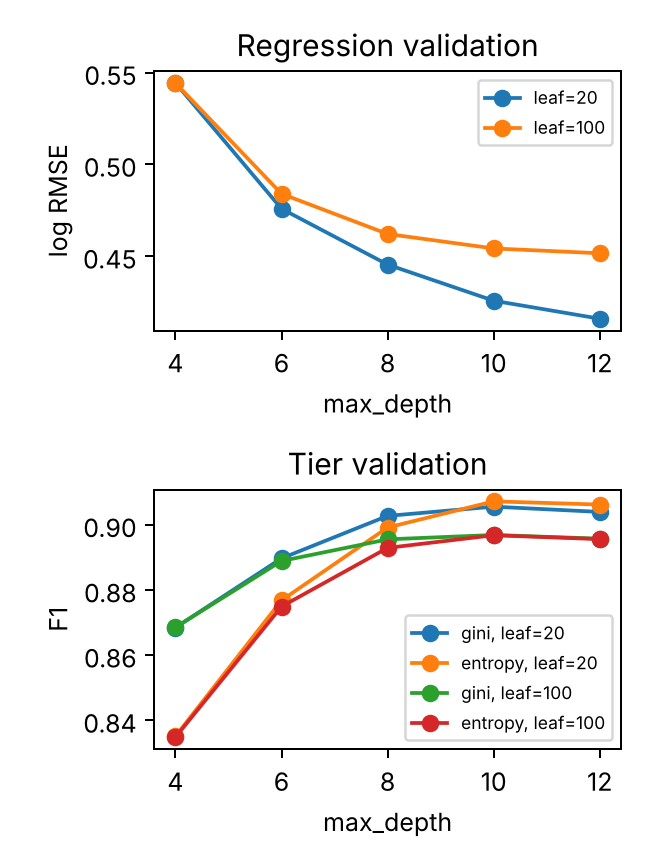
\includegraphics[width=\linewidth]{figures/tree_validation_report.png}
  \caption{Decision-tree validation curves used for configuration
  selection. Lower is better for regression log-RMSE; higher is better
  for classification F1.}
  \label{fig:validation}
\end{figure}

The linear Pegasos model learned $\|w\|=1.501$ and a margin width of
$2/\|w\|=1.332$ in standardised feature space. By the criterion
$y_i(w^\top x_i+b)\leq1$, 37,186 of 45,118 training rows were support
vectors. Its regularised hinge objective fell from 12.676 after 100
updates to 0.797 after 20,000 updates, with small stochastic fluctuations.

Price errors were much larger in the luxury tail. The 85 test listings
above the training 99th-percentile price of 2.5 million AZN had mean
absolute error 3.65 million AZN, versus 74.5 thousand AZN for the
remaining 9,584 test listings. The median absolute error across the
whole test set was 26.0 thousand AZN. Our tree underpredicted 89.4\%
of those 85 tail listings, indicating systematic compression of high
prices. The reproducible run also saves a log-scale actual-versus-predicted
plot for detailed inspection.

\section{Discussion and Limitations}
Where and why each model fails (luxury outliers, sparse districts,
scaling effects), the bias--variance story, and honest limitations.

\section{Conclusion}
One short paragraph: what you found and what you would do next.

\section*{Tools and Acknowledgements}
An AI coding assistant helped draft and test the integration runner,
evaluation metrics, baseline comparisons, README, and this Results
section. The dataset came from the Kaggle source~\cite{binaaz};
scikit-learn was used only for comparison models and
metric cross-checks. Team members should verify the final report and
record their individual contributions before submission.

% =====================================================================
\begin{thebibliography}{9}
\bibitem{pegasos}
S.~Shalev-Shwartz, Y.~Singer, N.~Srebro, and A.~Cotter,
``Pegasos: primal estimated sub-gradient solver for SVM,''
\emph{Mathematical Programming}, vol.~127, no.~1, pp.~3--30, 2011.
\bibitem{binaaz}
sehriyarmemmedli, ``Binaaz sale project,'' Kaggle, dataset version 1.
\href{https://www.kaggle.com/datasets/sehriyarmemmedli/binaaz-sale-project}{Dataset page}
(accessed Oct.~15, 2026).
\end{thebibliography}

\end{document}
